
% --------------------------------------------------------------
% This is all preamble stuff that you don't have to worry about.
% Head down to where it says "Start here"
% --------------------------------------------------------------
 
\documentclass[12pt]{article}
 
\usepackage[margin=1in]{geometry} 
\usepackage{amsmath,amsthm,amssymb}
 
\usepackage{listings}
\lstset{
basicstyle=\small\ttfamily,
columns=flexible,
breaklines=true
} 
 
\usepackage{graphics,amsfonts}
\usepackage{epstopdf}
\usepackage[pdftex]{graphicx}
\usepackage{float}
\usepackage{scrextend}
 
\newcommand{\N}{\mathbb{N}}
\newcommand{\Z}{\mathbb{Z}}
 
\newenvironment{theorem}[2][Theorem]{\begin{trivlist}
\item[\hskip \labelsep {\bfseries #1}\hskip \labelsep {\bfseries #2.}]}{\end{trivlist}}
\newenvironment{lemma}[2][Lemma]{\begin{trivlist}
\item[\hskip \labelsep {\bfseries #1}\hskip \labelsep {\bfseries #2.}]}{\end{trivlist}}
\newenvironment{exercise}[2][Exercise]{\begin{trivlist}
\item[\hskip \labelsep {\bfseries #1}\hskip \labelsep {\bfseries #2.}]}{\end{trivlist}}
\newenvironment{reflection}[2][Reflection]{\begin{trivlist}
\item[\hskip \labelsep {\bfseries #1}\hskip \labelsep {\bfseries #2.}]}{\end{trivlist}}
\newenvironment{proposition}[2][Proposition]{\begin{trivlist}
\item[\hskip \labelsep {\bfseries #1}\hskip \labelsep {\bfseries #2.}]}{\end{trivlist}}
\newenvironment{corollary}[2][Corollary]{\begin{trivlist}
\item[\hskip \labelsep {\bfseries #1}\hskip \labelsep {\bfseries #2.}]}{\end{trivlist}}
 
\usepackage{blindtext} % for dummy text

\makeatletter
    \setlength\@fptop{0\p@}
\makeatother

\begin{document}
 
% --------------------------------------------------------------
%                         Start here
% --------------------------------------------------------------
 
%\renewcommand{\qedsymbol}{\filledbox}
 
\title{COMPUTER VISION – Project 1
Autonomous Driving: Road Sign Recognition}%replace X with the appropriate number
\author{Carlo Rizzardo - 1156404\\ %replace with your name
Computer Vision} %if necessary, replace with your course title
 
\maketitle


The solution to the proposed problem consists in the \textit{StreetSignsIdentifier} class, the objects of this class, once set up, allow to identify the road sign in the provided images.
The public interface of the class consists just in the constructor, a utility method for setting the verbosity for the whole object and
the \textit{identify(cv::Mat\& img)} method. This last method receives an image in input and returns a list of \textit{StreetSign} objects containing all the traffic signs which have been detected in the image. The \textit{StreetSign} object is a superclass for the objects \textit{StreetSign\_Warning}, \textit{StreetSign\_NoParking} and \textit{StreetSign\_Speed}, which represent 
more specific types of signs. From each of these object it is possible to get the location of the sign  in the image and, in the case of the speed limits, the maximum speed allowed by the sign.
The actual detection and classification is performed using a variety of different methods. The first approach is the usage of two cascade classifiers, one for the triangular warning signs and the other one for all the round red signs.
After this first detection the algorithm proceeds to create a mask representing the red areas in the image, this is done by two different method whose results are then intersected. The first one uses a distance function based on the hue and then
multiplied by the saturation, which when thresholded provides a first mask, the other one uses a distance function based on the lab color space. Both these methods are applied to a subsampling of the image for performance reasons.
The mask is then used to confirm the detections from the cascade classifiers, only the detections whose area contain at least 5\% of red pixels are kept.
After this the warning signs are identified, but the round ones need a further classification into speed limits or no-parking signs. This is done first by recognizing as no-parking signs the signs which have at least a line that passes near the origin with an orientation of about 135 degrees.
This detection is done using Hough on an edge image computed using the Canny edge detector. The remaining signs are then searched for digits, this is done performing first a threshold of the sign, followed by a computation of the contours and their bounding boxes. These boxes are then filtered by their sizes and in them are detected the digits using a \textit{kNearestNeighbor} classifier, which is trained with an image that can be found in the template folder.

The training of the cascades has been done on a mix of samples form the BelgiumTS Belgium Traffic signs Dataset and the German 
Traffic sign dataset. Ultimately with 1800 positive samples for the warning signs and 1250 for the round ones.


\begin{figure}[ht!]
	\centering
 	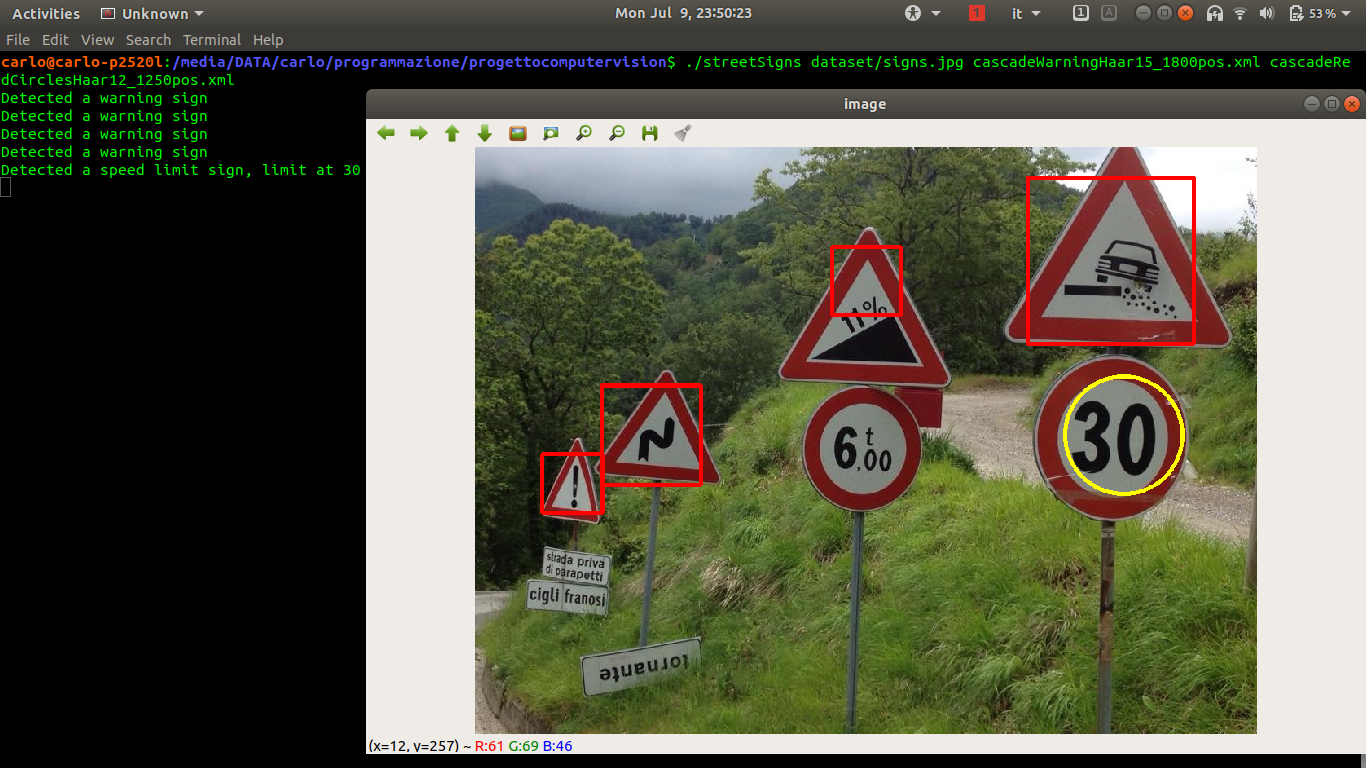
\includegraphics[scale = 0.35]{./Screenshot20180709_235023}
	\caption{ The result of the algorithm on the dataset/signs.jpg image}
\end{figure}
 
 \begin{figure}[ht!]
	\centering
 	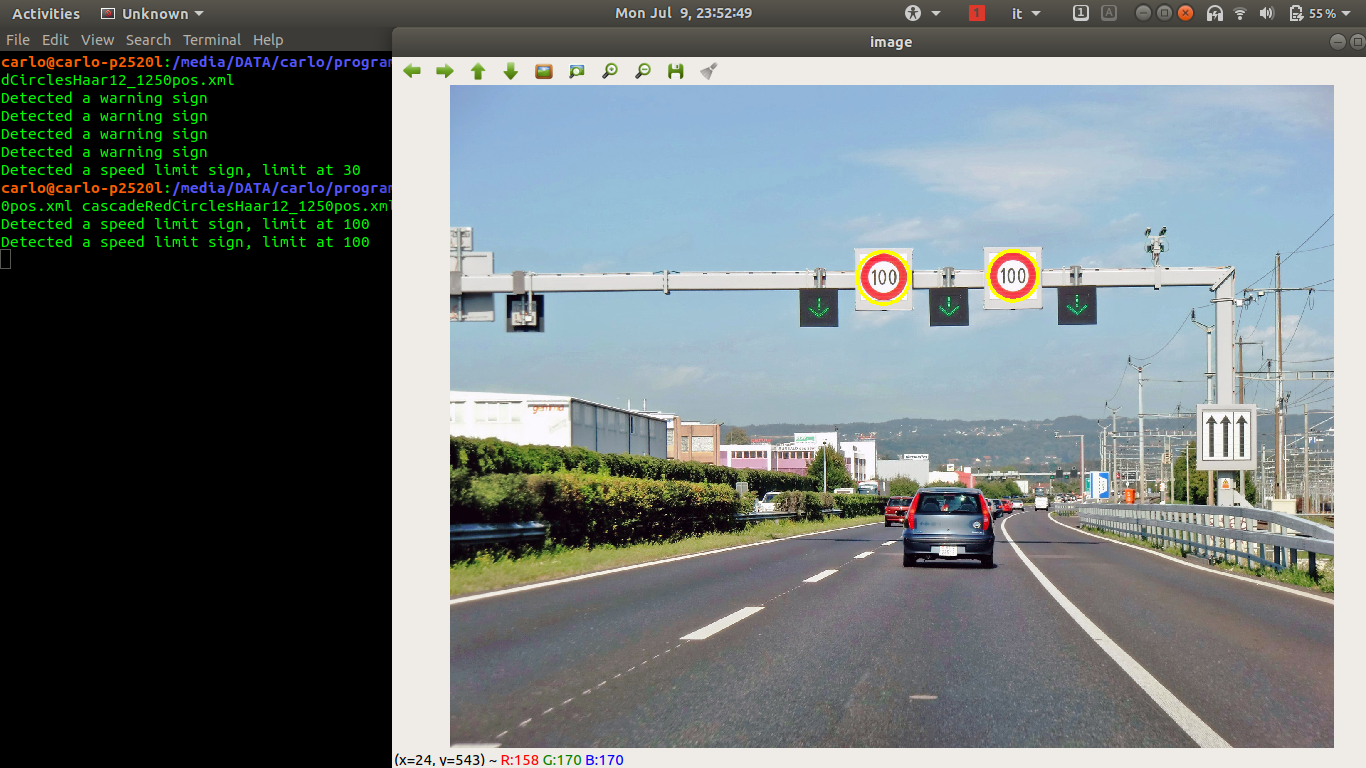
\includegraphics[scale = 0.35]{./Screenshot2018-07-0923-52-48}
	\caption{ The result of the algorithm on the dataset/dataset/562421b3b5e3f2-18253398.jpg image}
\end{figure}

\end{document}
              
